%\documentclass[aps,onecolumn,preprint,superscriptaddress,nofootinbib,floats]{revtex4}
%\usepackage{graphicx}

\documentclass[12pt]{article}

\usepackage{amsmath}
\usepackage[linesnumbered,ruled,noline,noend]{algorithm2e}

%\usepackage[linesnumbered,noline,noend]{algorithm2e}
%\usepackage{amsmath}

\SetNlSty{}{}{}

\let\oldnl\nl% Store \nl in \oldnl
\newcommand\nonl{%
  \renewcommand{\nl}{\let\nl\oldnl}}% Remove line number for one line



\def\beq{\begin{equation}}
\def\eeq{\end{equation}}


\usepackage{amsmath,amssymb,graphicx,multirow,xspace,slashed}
\usepackage[colorlinks=true,urlcolor=blue,anchorcolor=blue,citecolor=blue,filecolor=blue,linkcolor=blue,menucolor=blue,pagecolor=blue]{hyperref}


\usepackage{floatrow}
% Table float box with bottom caption, box width adjusted to content
\newfloatcommand{capbtabbox}{table}[][\FBwidth]


\usepackage[font=footnotesize,labelfont=bf]{caption}

\newcommand*\myat{{\fontfamily{ptm}\selectfont @}}

%\usepackage[notref]{showkeys}
\usepackage{lineno}

\allowdisplaybreaks
%\bibliographystyle{JHEP}

\addtolength{\oddsidemargin}{-.4in}
\addtolength{\evensidemargin}{-.4in}
\addtolength{\textwidth}{0.8in}
\addtolength{\topmargin}{-.6in}
\addtolength{\textheight}{1in}
%\addtolength{\footskip}{0.3in}
\renewcommand{\baselinestretch}{1.2}

\long\def\symbolfootnote[#1]#2{\begingroup%
\def\thefootnote{\fnsymbol{footnote}}\footnote[#1]{#2}\endgroup}

\renewcommand{\textfraction}{0}
\renewcommand{\topfraction}{0.95}


\newcommand{\newc}{\newcommand}
\newc{\gsim}{\lower.7ex\hbox{$\;\stackrel{\textstyle>}{\sim}\;$}}
\newc{\lsim}{\lower.7ex\hbox{$\;\stackrel{\textstyle<}{\sim}\;$}}
\newc{\gev}{\,{\rm GeV}}
\newc{\mev}{\,{\rm MeV}}
\newc{\ev}{\,{\rm eV}}
\newc{\kev}{\,{\rm keV}}
\newc{\tev}{\,{\rm TeV}}

\newcommand{\ifb}{\,\mathrm{fb}^{-1}}
\newcommand{\ipb}{\,\mathrm{pb}^{-1}}
\renewcommand*\descriptionlabel[1]{\hspace\labelsep\normalfont #1}

\def\ln{\mathop{\rm ln}}
\def\tr{\mathop{\rm tr}}
\def\Tr{\mathop{\rm Tr}}
\def\Im{\mathop{\rm Im}}
\def\Re{\mathop{\rm Re}}
\def\bR{\mathop{\bf R}}
\def\bC{\mathop{\bf C}}
\def\lie{\mathop{\hbox{\it\$}}} %pound sterling
\newc{\mz}{M_Z}
\newc{\mpl}{M_*}
\newc{\mw}{m_{\rm weak}}
\newc{\nr}[1]{N^c_R{}_{#1}}

%\renewcommand{\phi}{\varphi}

%indices and other greek stuff
\renewcommand{\a}{\alpha}
\newcommand{\da}{{\dot \alpha}}
\renewcommand{\b}{\beta}
\newcommand{\db}{{\dot\beta}}
\newcommand{\g}{\gamma}
\newcommand{\dg}{{\dot\gamma}}
\renewcommand{\d}{\delta}
\newcommand{\dd}{{\dot\delta}}
\newcommand{\m}{\mu}
\newcommand{\n}{\nu}
\newcommand{\e}{\epsilon}
\newcommand{\s}{\sigma} 
\renewcommand{\r}{\rho}
\newcommand{\bs}{{\bar\sigma}}
\renewcommand{\l}{\lambda}
\renewcommand{\L}{\Lambda}
\renewcommand{\k}{\kappa}
\renewcommand{\th}{\theta}
\newcommand{\thb}{{\bar\theta}}
\newcommand{\D}{\Delta}
\newcommand{\B}{\bar B_\mu}
\newcommand{\cA}{c_{A_{u,d}}}
\newcommand{\cH}{c_{m_{u,d}}}
\renewcommand{\dag}{\dagger}
\newcommand{\bra}{\langle}
\newcommand{\ket}{\rangle}
\newcommand{\Q}{\bar Q}
\renewcommand{\O}{O}

\newcommand{\CM}{{\mathcal M}}

%%%%%%%%%%%%%%%%%%%%%%%% special abrev's %%%%%%%%%%%%%%%%%%%%%%%%%%%%%

\newcommand{\mhu}{{\hat m_{H_u}}}
\newcommand{\mhd}{{\hat m_{H_d}}}
\newcommand{\mhud}{{\hat m_{H_{u,d}}}}


%%%%%%%%%%%%%%%%%%%%%%% latex eqn abrev's %%%%%%%%%%%%%%%%%%%%%%%%%%%%

\def\beq{\begin{equation}}
\def\eeq{\end{equation}}
\newcommand{\bea}{\begin{eqnarray}\begin{aligned}}
\newcommand{\eea}{\end{aligned}\end{eqnarray}}
\def\bitem{\begin{itemize}}
\def\eitem{\end{itemize}}
%
%
%%%%%%%%%%%%%%%%%%%%%%% common abrev's %%%%%%%%%%%%%%%%%
%
%

\newc{\ie}{{\it i.e.}}          \newc{\etal}{{\it et al.}}
\newc{\eg}{{\it e.g.}}          \newc{\etc}{{\it etc.}}
\newc{\cf}{{\it c.f.}}
\newcommand{\kahler}{K\"{a}hler }

\newcommand{\lang}{\mathcal{L}}
\newcommand{\C}{\mathbb{C}}
\newcommand{\CO}{O}
\newcommand{\half}{\frac{1}{2}}


%\renewcommand{\epvar}{\varepsilon}
%\renewcommand{\phi}{\varphi}
\renewcommand{\topfraction}{0.85}
\renewcommand{\textfraction}{0.1}
\renewcommand{\floatpagefraction}{0.75}

%number equations by section
 %\numberwithin{equation}{section}

%toc depth
\setcounter{tocdepth}{2}

%Begin special definitions for Instructions file
\newcommand{\ttbs}{\char'134}%\backslash for \tt
\newcommand\fverb{\setbox\fverbbox=\hbox\bgroup\verb}
\newcommand\fverbdo{\egroup\medskip\noindent%
            \fbox{\unhbox\fverbbox}\ }
\newcommand\fverbit{\egroup\item[\fbox{\unhbox\fverbbox}]}
\newbox\fverbbox
\newcommand{\jhepname}{JHEP}
%end


\renewcommand{\arraystretch}{1.3}

%\usepackage[usenames,dvipsnames]{xcolor}


\usepackage{tikz}

\newcommand{\shrug}[1][]{%
\begin{tikzpicture}[baseline,x=0.8\ht\strutbox,y=0.8\ht\strutbox,line width=0.125ex,#1]
\def\arm{(-2.5,0.95) to (-2,0.95) (-1.9,1) to (-1.5,0) (-1.35,0) to (-0.8,0)};
\draw \arm;
\draw[xscale=-1] \arm;
\def\headpart{(0.6,0) arc[start angle=-40, end angle=40,x radius=0.6,y radius=0.8]};
\draw \headpart;
\draw[xscale=-1] \headpart;
\def\eye{(-0.075,0.15) .. controls (0.02,0) .. (0.075,-0.15)};
\draw[shift={(-0.3,0.8)}] \eye;
\draw[shift={(0,0.85)}] \eye;
% draw mouth
\draw (-0.1,0.2) to [out=15,in=-100] (0.4,0.95); 
\end{tikzpicture}}



\newcommand{\MYhref}[3][blue]{\href{#2}{\color{#1}{#3}}}%

\begin{document}
%
%\title{Toy Generative Model for Jets}
%\author{Kyle Cranmer, Sebastian Macaluso and Duccio Pappadopulo}
%\maketitle


\begin{center}

\vskip 1cm
{\Large \bf  Tree Clustering Algorithms for Jets Physics}

\vskip 1.0cm
{\large $\text{Kyle Cranmer}^1$, $\text{Sebastian Macaluso}^1$ and $\text{Duccio Pappadopulo}^2$}
\vskip 0.6cm
{\small \it 1 Center for Cosmology and Particle Physics $\&$ Center for Data Science, New York University, USA} \\
{\small \it 2 Bloomberg LP, New York, NY 10022, USA.}
\vskip 2.0cm

\end{center}




\section{Motivation and problem formulation}
 
 
At physics colliders, e.g. the Large Hadron Collider at CERN, two beams of particles (accelerated to very high energies) directed against each other are collided head-on. As a result, new unstable particles get created and a {\it showering process} happens, where successive binary splittings of these initial unstable particles are produced until all the particles are stable. This process gives rise to jets, which are a collimated spray of energetic charged and neutral particles. We refer to these final particles as the jet constituents.
 
 As a result of this showering process, there could be many latent paths that may lead to a specific jet (i.e. the set of constituents). Thus, it is natural to represent a jet and the particular showering path that gave rise to it as a binary tree, where the inner nodes represent each of the unstable particles and the leaves represent the jet constituents.   
 
 In this context, it becomes relevant and interesting to study algorithms to reconstruct the jet constituents (leaves) into a binary tree (clustering algorithms) and how close these algorithms can reconstruct the truth latent path. Being able to perform a precise reconstruction of the truth tree would assist in physics searches at the Large Hadron Collider. In particular, determining the nature (type) of the initial unstable particle (and its children and grandchildren) that gave rise to a specific jet is essential in searches of new physics as well as precision measurements of the current model, i.e. the Standard Model of Particle Physics.
 
 There are software tools called {\bf parton showers}, e.g. \MYhref{http://home.thep.lu.se/Pythia/}{PYTHIA}, \MYhref{https://herwig.hepforge.org/}{Herwig}, \MYhref{https://sherpa.hepforge.org/trac/wiki}{Sherpa}, that encode a physics model for the simulation of jets that are produced at colliders. Currently, parton shower generators in full physics simulations are implicit models, i.e. they are a probabilistic model defined only in terms of the samples they generate. Thus, the likelihood of a particular showering process is intractable. As a result, to aid in machine learning (ML) research for jet physics, a python package for a toy generative model of a parton shower was provided in \cite{ToyJetsShowerPackage}. This model has a tractable likelihood, and is as simple and easy to describe as possible but at the same time captures the essential ingredients of parton shower generators in full physics simulations (see \cite{ToyJetsShower} for more details).
 
In particle physics collisions, the likelihood $p(x| \theta) $ for parameters $\theta$ defined in the physics model given data $x$, can be factorized into a parton level-process, a parton shower and detector interactions, as introduced in \cite{Brehmer:2018kdj}.  


\beq
p(x|\theta) = \int dz_{\text{detector}} \int dz_{\text{shower}} \int dz \,p(x|z_{\text{detector}})  p(z_{\text{detector}}| z_{\text{shower}})  p(z_{\text{shower}}|z,\theta_s) p(z|\theta_t)
\eeq

where each term in the integral describes the likelihood of a latent path $z$ given the model parameters $\{\theta_t,\,\theta_s\}$. In particular, $p(z|\theta_p)$ is the likelihood of getting matrix element level momenta $z$ conditional on the theory parameters $\theta_t$, and $p(z_{\text{shower}}|z,\theta_s)$ the likelihood of a particular showering history conditional on $z$ and shower model parameters $\theta_s$. Also, $p(z_{\text{detector}}| z_{\text{shower}})$ and $p(x|z_{\text{detector}})$ describe how the process evolves to reconstructed observables $x$ through detector effects and the reconstruction method, respectively.

In this work we are interested in studying how well we can reconstruct the joint likelihood $p(z_{\text{shower}}|z,\theta_s)$ for a given shower history $z_{\text{shower}}$ (tree latent path) of a jet, as we show schematically in fig. \ref{fig:treestructure}. Thus, we will focus on the showering likelihood and for our purposes we will consider the final states of the shower as the observables $x$.\footnote{We leave the study of detector and reconstruction effects for future work. Also, for simplicity we do not include hadronization effects.}


\begin{figure*}
{
  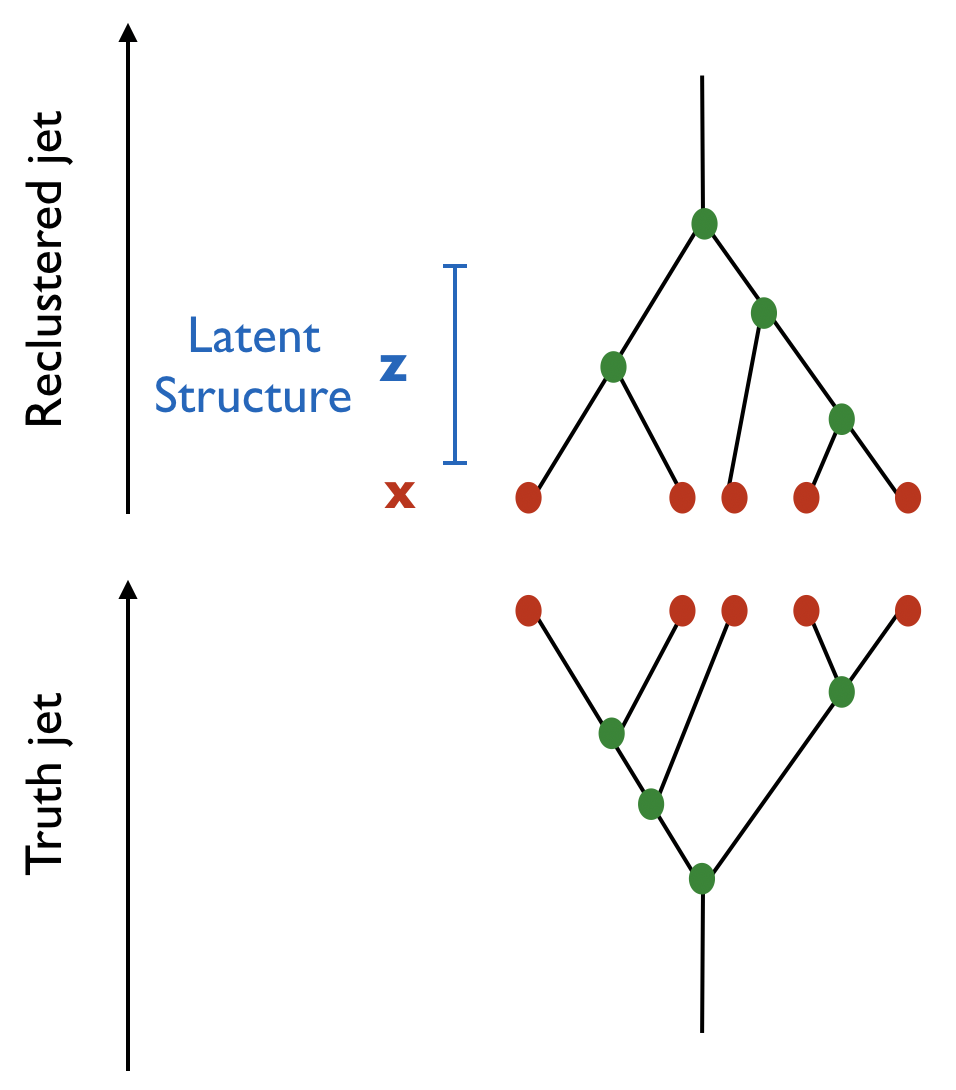
\includegraphics[width=0.4\linewidth]{plots/JetLatentStructure.png}
}
\caption{\small{Schematic representation of the tree structure of a sample jet generated with our Toy Model for Jets and the reclustered tree for some clustering algorithm. For a given algorithm, $z$ labels the different variables that determine the latent structure of the tree. The tree leaves $x$ are labeled in red and the inner nodes in green. 
}}
\label{fig:treestructure}
\end{figure*}

Traditionally, jets are generated with a parton shower and then one of the generalized $k_t$ clustering algorithms is used to reconstruct them. These algorithms sequentially cluster jet constituents by merging the closest pair based on a distance measure:
\beq\label{eq:dij}
d_{ij}=\text{min}(p_{ti}^{2 \alpha},p_{tj}^{2 \alpha}) \frac{\Delta R_{ij}^2}{R^2}
\eeq
where $\Delta R_{ij}$ is the angular distance for the pair $\{i,j\}$, $R$ is a fixed value for the jet radius and  $\alpha = \{-1,0,1\}$ specifies the anti-$k_t$, Cambridge/Aachen and $k_t$ algorithms respectively.

The Toy Generative Model for Jets enables us to explore and compare different jet clustering algorithms based on the jet likelihood, given that we can reconstruct  $p(z_{\text{shower}}|z,\theta_s) $. As a result, this model allows to have a unified picture for generation and inference, and could lead to a systematic fit of shower parameters $\theta_s$ to data, following the technique introduced in \cite{Brehmer:2018kdj}.
 
%In fig. \ref{fig:treestructure} we show a schematic representation of the tree structure of a sample jet generated with our Toy Model for Jets and the reclustered tree for some clustering algorithm. For a given algorithm, $z$ labels the different variables that determine the latent structure of the tree.  

 % =====================================================
\vspace{0.6cm}
 \section{Likelihood-based clustering algorithms}

% This package implements different algorithms to recluster a set of jet constituents (leaves) into a binary tree.
% In particular, we explore how different algorithms can reconstruct the latent structure of the jets generated with the [`Toy Generative Model for Jets`](https://github.com/SebastianMacaluso/ToyJetsShower) package.  Comparisons and visualizations are enabled thanks to the   [`VisualizeBinaryTrees`](https://github.com/SebastianMacaluso/VisualizeBinaryTrees) package (also included within this package for ease of use).
 
% 
% There can be many techniques to recluster the set of jet constituents (leaves) into a binary tree, from machine learning based ones to more traditional algorithms. In this package, first we implement the traditional physics based generalized $k_t$ clustering algorithms on the jets generated with the [`Toy Generative Model for Jets`](https://github.com/SebastianMacaluso/ToyJetsShower). These algorithms, which will be used for comparison, are characterized by:
% 
% - Permutation invariance with respect to the order in which we cluster the jet constituents. 
%
%- Distance measure: the angular separation between two jet constituents is typically used as a distance measure among them. In particular, traditional jet clustering algorithms are based on a measure given by $d_{ij} ~  Delta R_{ij}^2$, where $Delta R_{ij}$ is the angular separation between two particles.

 There can be many techniques to cluster the set of jet constituents (leaves) into a binary tree, from machine learning based ones to more traditional algorithms.
 
\subsection{Maximum likelihood estimate} 
 
 We start by studying algorithms that aim to maximize the joint likelihood of a jet. Thus, we want to find the maximum likelihood estimate (MLE) for the latent structure of a jet, given a set of leaves. In this approach, the tree latent structure $z_{\text{shower}}$ is fixed by the algorithm we choose. Also, as already mentioned, for our purposes we will consider the final states of the shower as the observables $x$. A complete solution can be found using the Viterbi algorithm, obtaining $\hat{z}_{\text{Viterbi}} = \text{argmax}_{z_{\text{shower}}}   \,p(x | z_{\text{shower}}) $. However, this approach becomes computationally infeasible for a large number of leaves, e.g. we typically consider jets with 50 to 100 constituents.
There are other algorithms that provide an approximate solution, i.e. greedy and beam search algorithms.

\begin{itemize}
\item Greedy Likelihood: tree joint likelihood $\hat{z}_{\text{Greedy}}$ from locally maximizing the likelihood of a node pairing at each step.  

\item Beam Search Likelihood: tree joint likelihood $\hat{z}_{\text{BS}}$ from maximizing the likelihood of multiple steps before choosing the latent path.

\end{itemize}

 
Next, in \cite{TreeAlgorithms} we introduce implementations of the greedy and beam search algorithms to jets physics and study how well they reconstruct the truth joint likelihood and latent structure of jets generated with the Toy Model. Visualizations to compare the latent structure are obtained using the python package in \cite{VisualizeBinaryTrees}.


Below we compare visualizations of the same sample jet (with 50 constituents) for the truth-level, greedy and beam search trees. First, in fig. \ref{fig:1Dtree70} we show three 1D tree-only visualizations where each node is connected to its parent. In each of the three cases, we compare the truth-level tree (bottom) versus the one we get with a clustering algorithm. Typically we expect that the fewer the lines crossings, the closer the latent structure to the truth tree. From this point of view, we could order the algorithms in increasing performance as $k_t$, greedy and beam search.
Next, in fig. \ref{fig:2Dclustermap70} we show 2D heat clustermaps where the color scale specifies the total number of steps needed to connect two leaves through their closest common ancestor using the truth-level jet tree. We show the leaves (and tree latent structure) ordered following the truth-level tree for columns and a clustering algorithm for rows (except for the bottom right heat map, where both columns and row represent the truth-level tree). The better the truth tree latent structure is reconstructed, the more the heat map structure looks block diagonal, as in the bottom right subfigure.
 
\begin{figure*}
\centering
\begin{minipage}[c]{0.49\textwidth}
 	 {
	  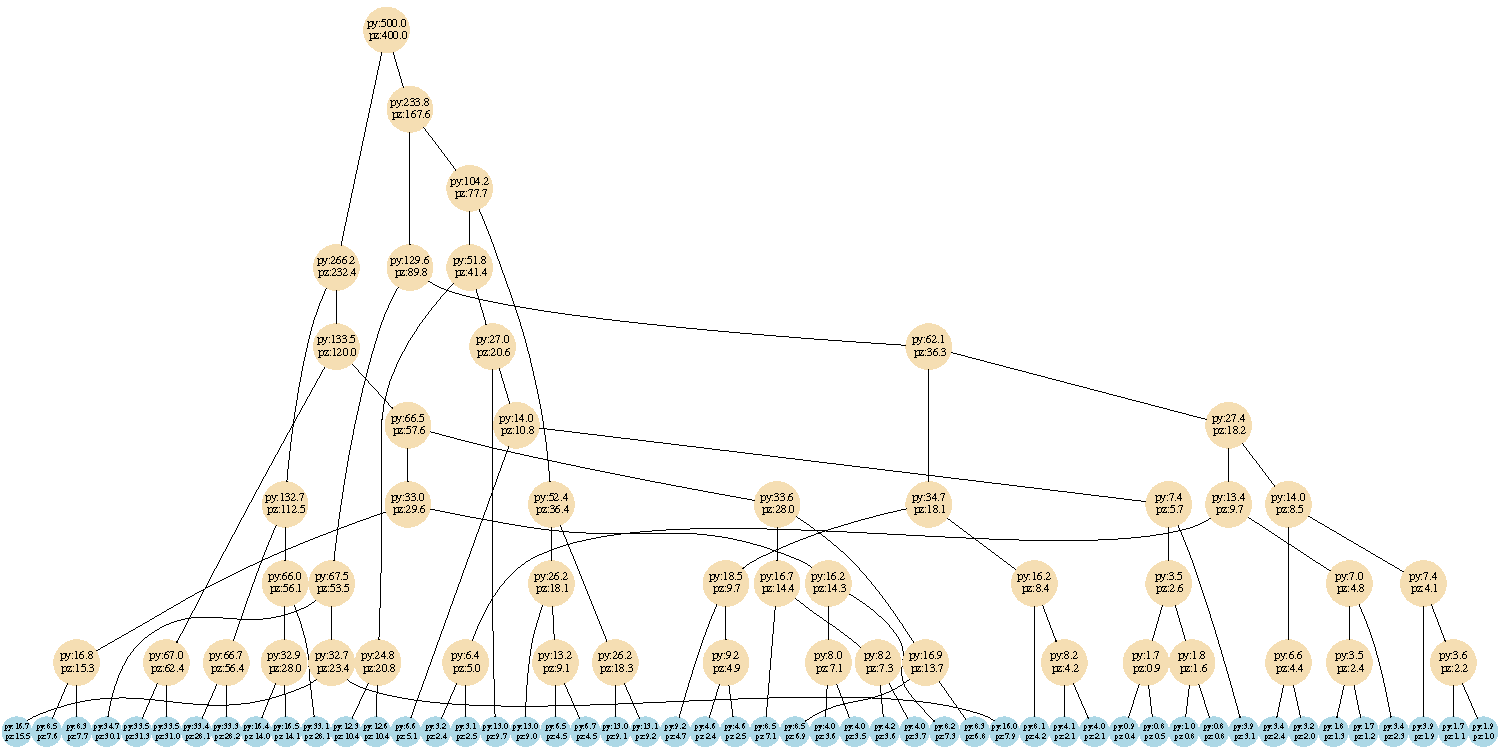
\includegraphics[width=\textwidth]{plots/jet70BS_orderTruth.pdf}
	   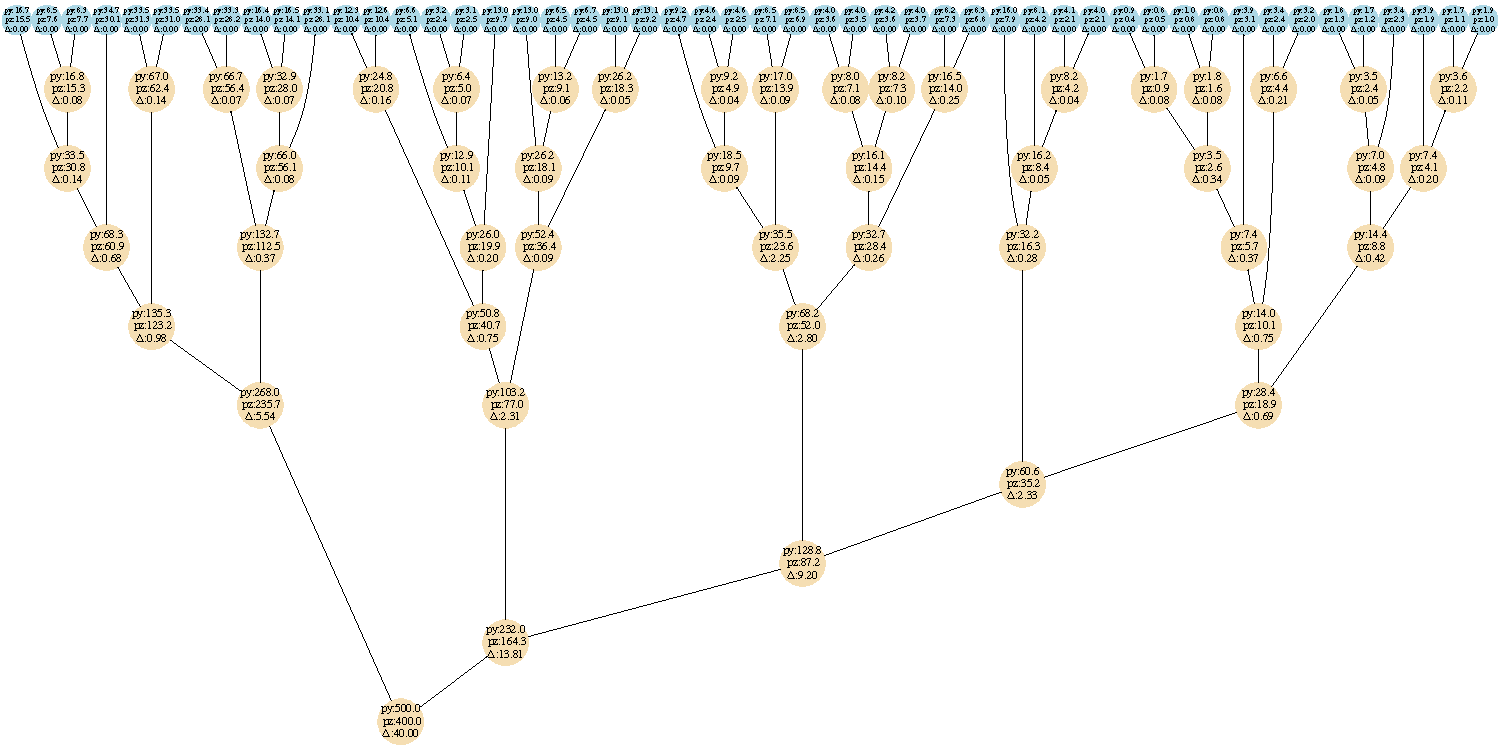
\includegraphics[width=\textwidth]{plots/jet70Truth_orderTruth.pdf}
	}
\end{minipage}
\begin{minipage}[c]{0.49\textwidth}
 	 {
	  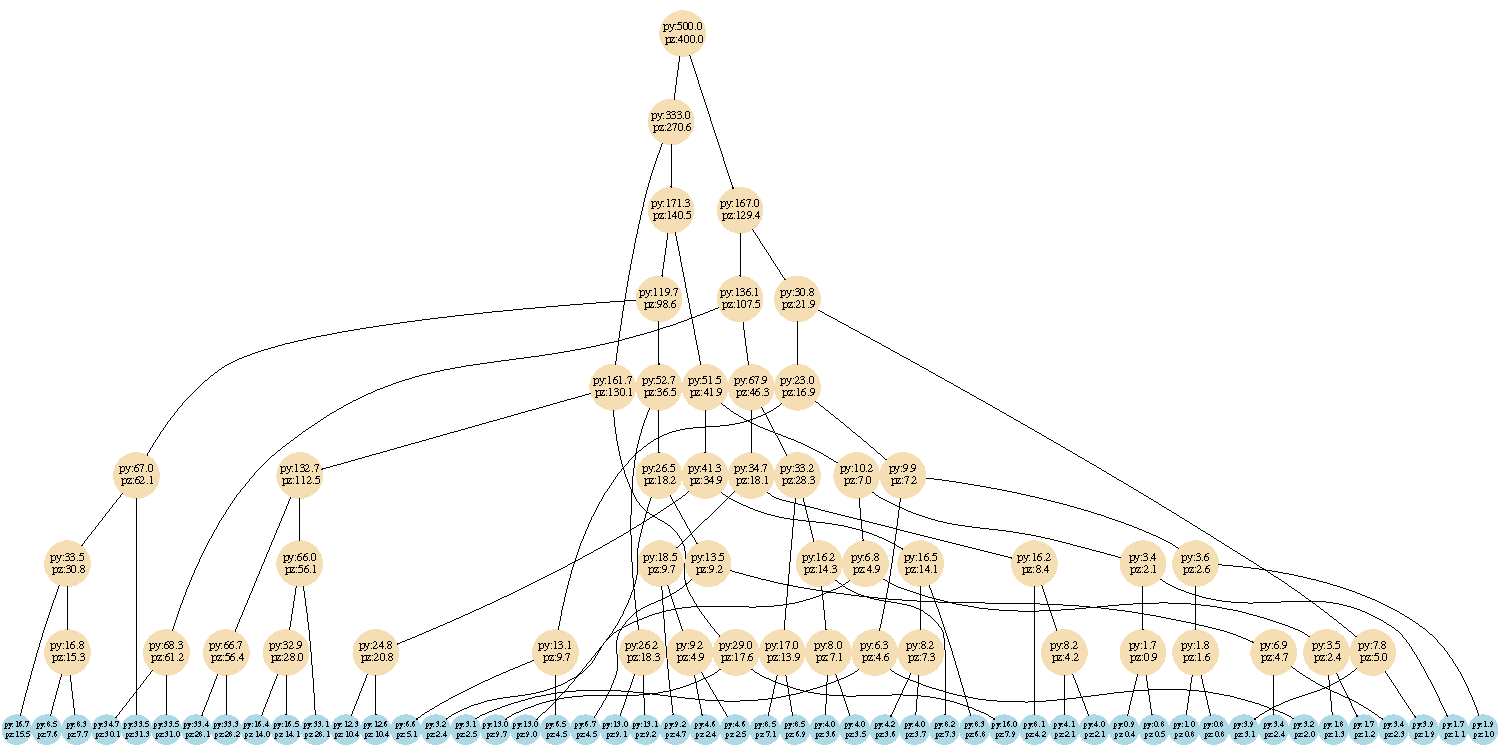
\includegraphics[width=\textwidth]{plots/jet70Greedy_orderTruth.pdf}
	   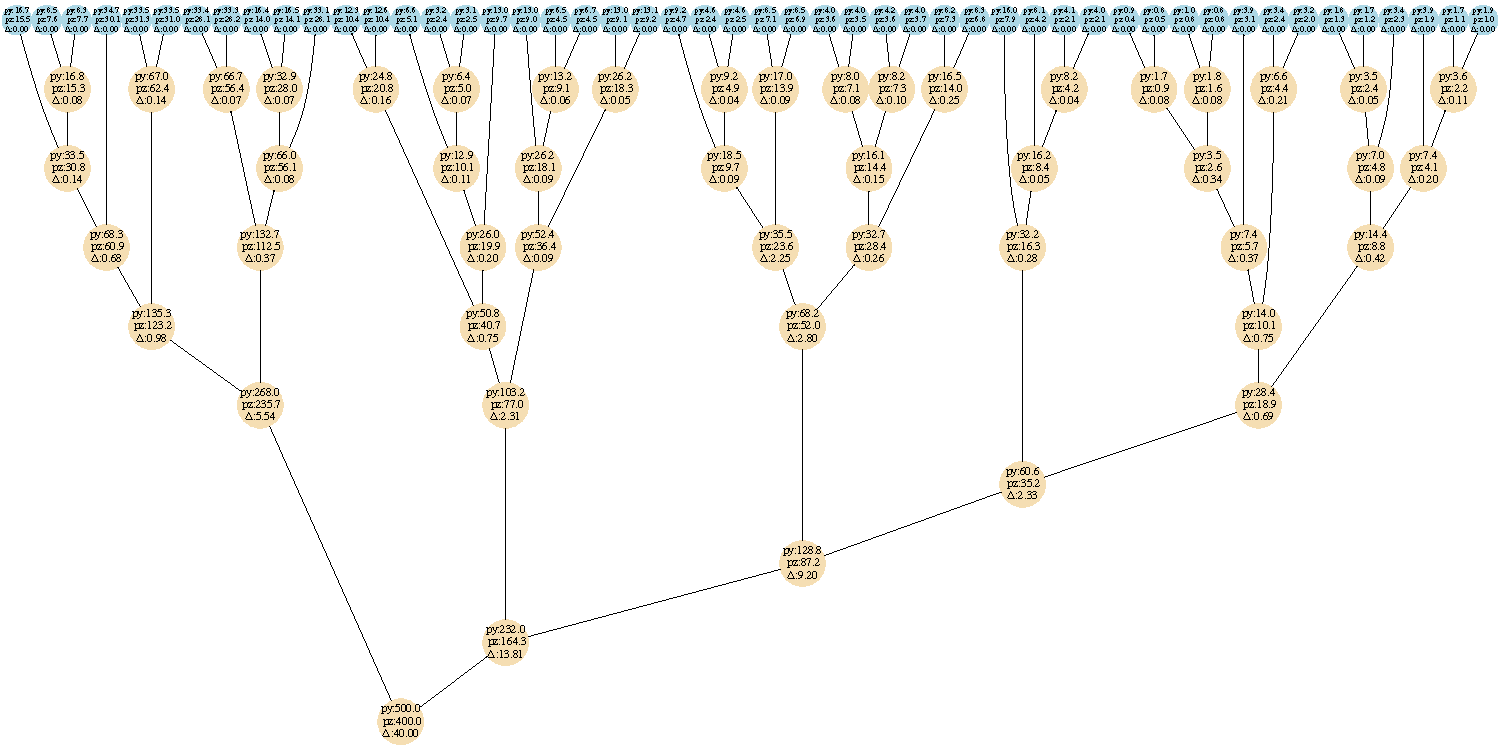
\includegraphics[width=\textwidth]{plots/jet70Truth_orderTruth.pdf}
	}
\end{minipage}
\begin{minipage}[c]{0.49\textwidth}
 	 {
	  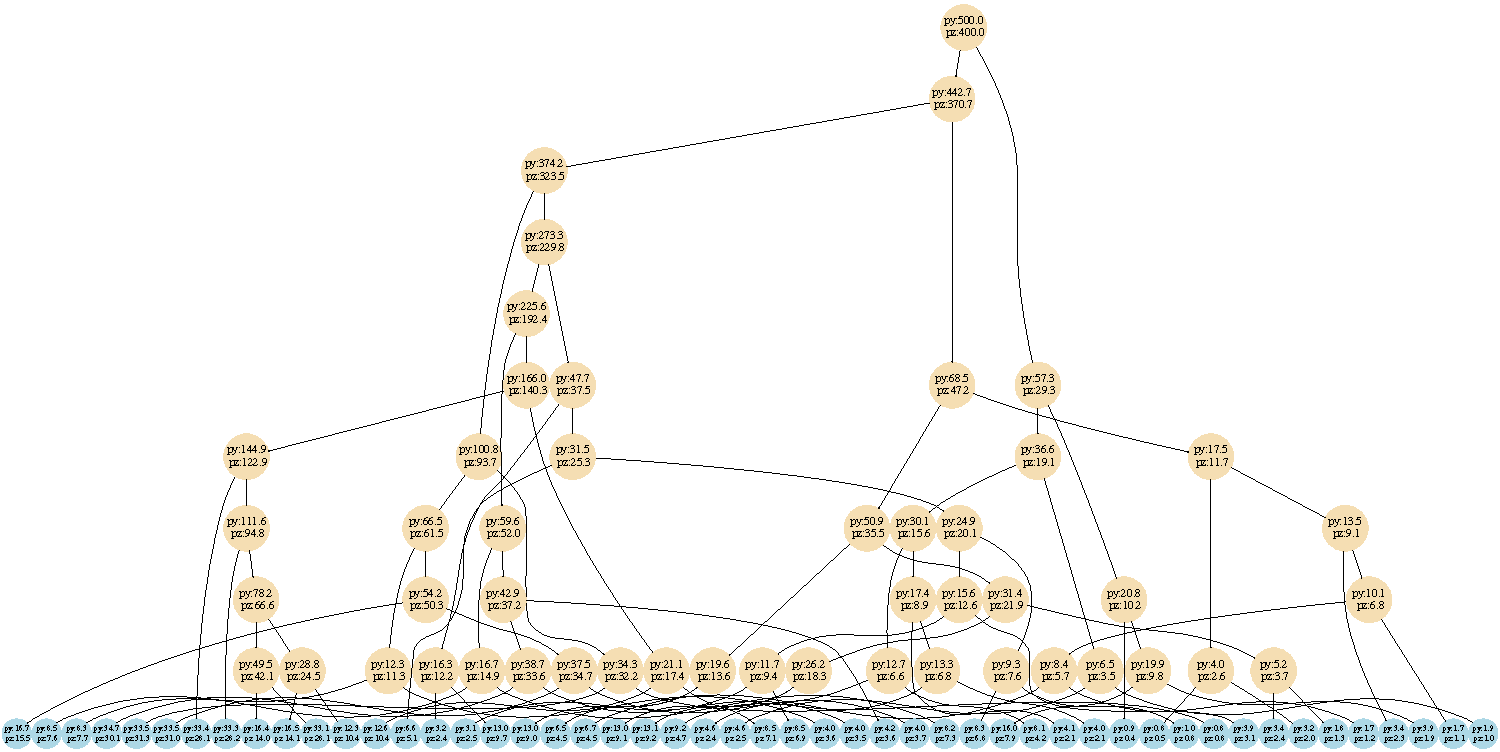
\includegraphics[width=\textwidth]{plots/jet70kt_orderTruth.pdf}
	   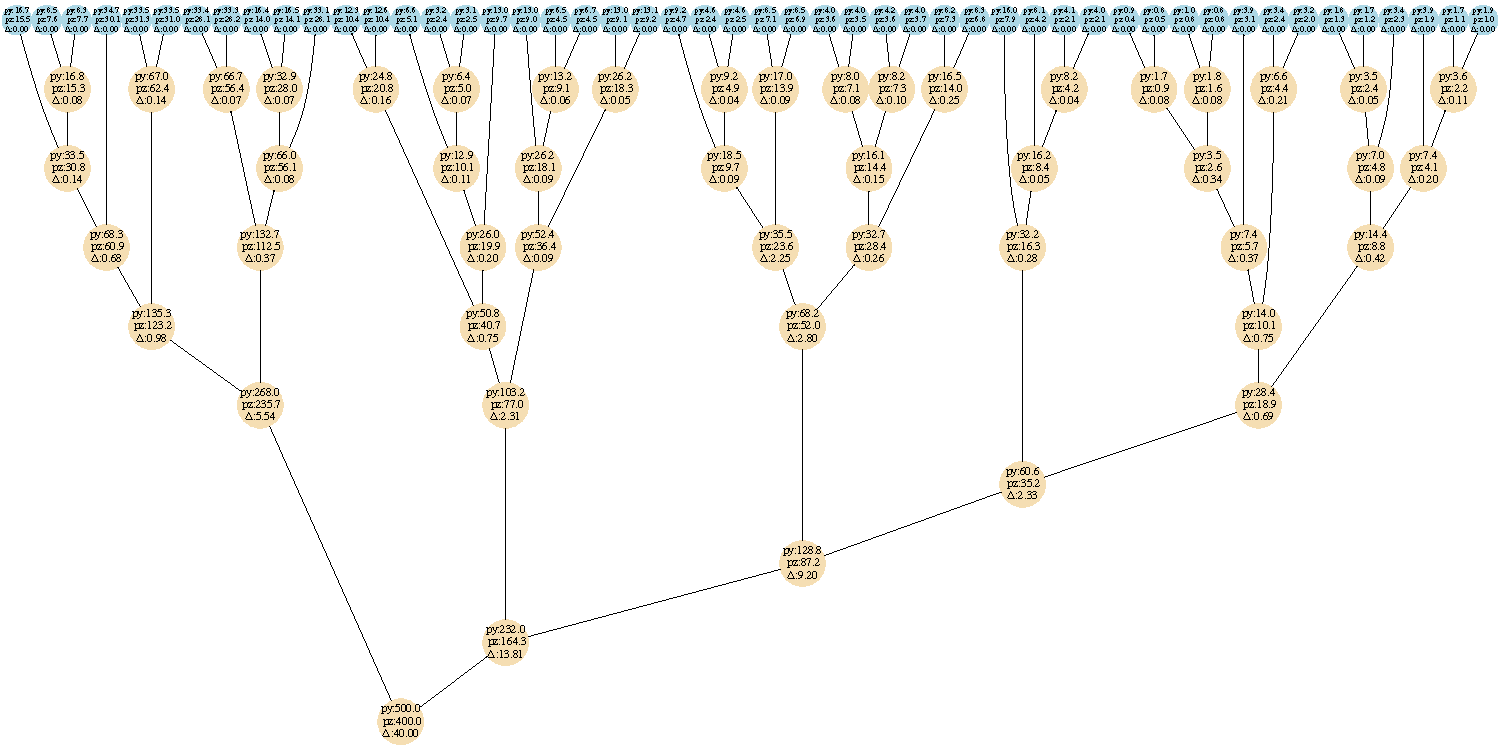
\includegraphics[width=\textwidth]{plots/jet70Truth_orderTruth.pdf}
	}
\end{minipage}
\caption{\small{1D Tree-only visualization of the same jet constituents reconstructed with three different algorithms, where we show the reclustered jet on top and the truth one at the bottom. Figures correspond to beam search (top left), greedy (top right) and $k_t$ (bottom) algorithms. The fewer the line crossings, the closer the latent structure is to the truth tree. The horizontal ordering of the leaves corresponds to the order in which the leaves are accessed when traversing the truth tree. 
}}
\label{fig:1Dtree70}
\end{figure*}






\begin{figure*}
\centering
\begin{minipage}[c]{0.49\textwidth}
 	 {
	  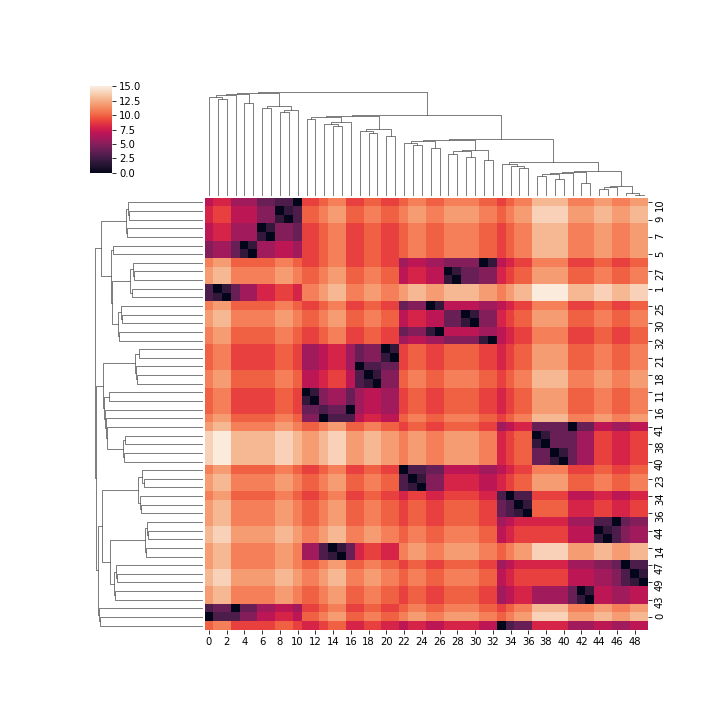
\includegraphics[width=\textwidth]{plots/jet70TrueHeatMap_orderBS.png}
	}
\end{minipage}
\begin{minipage}[c]{0.49\textwidth}
 	 {
	  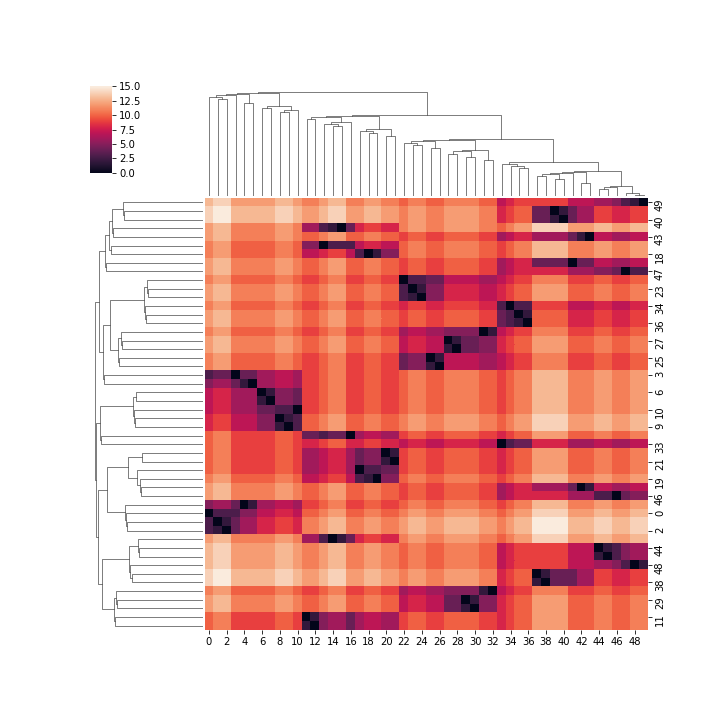
\includegraphics[width=\textwidth]{plots/jet70TrueHeatMap_orderGreedy.png}
	}
\end{minipage}
\begin{minipage}[c]{0.49\textwidth}
 	 {
	  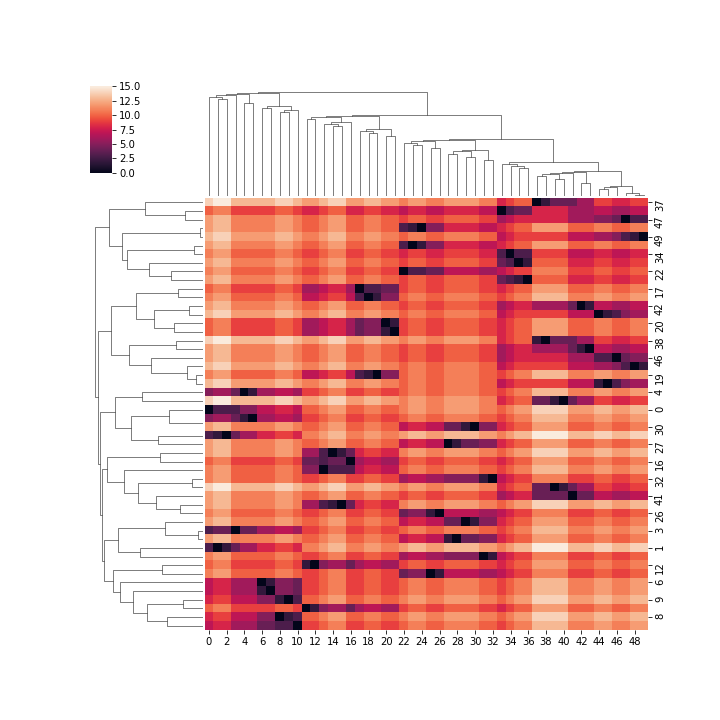
\includegraphics[width=\textwidth]{plots/jet70TrueHeatMap_orderkt.png}
	}
\end{minipage}
\begin{minipage}[c]{0.49\textwidth}
 	 {
	  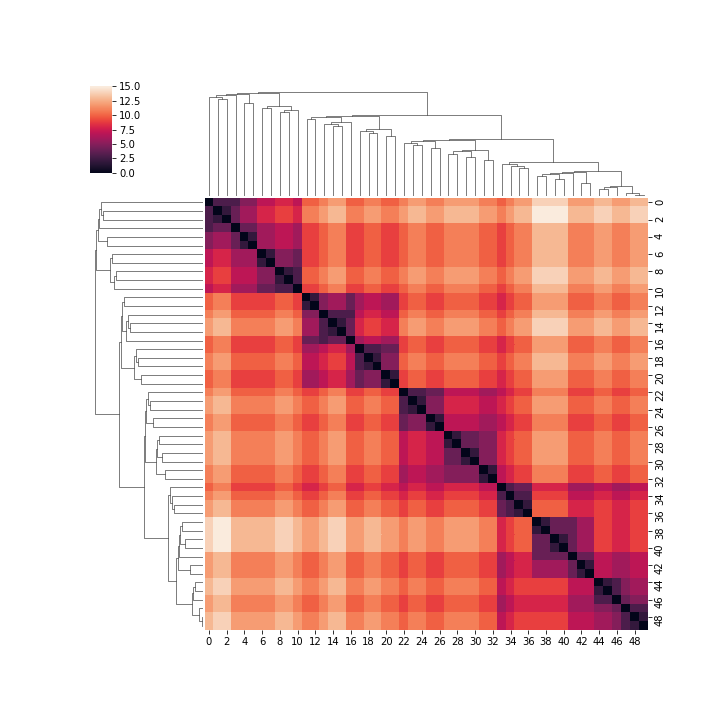
\includegraphics[width=\textwidth]{plots/jet70TrueHeatMap_orderTruth.png}
	}
\end{minipage}
\caption{\small{2D heat clustermap visualizations of the same truth jet. The leaves ordering corresponds to the order that they are accessed when traversing the truth tree (columns) and the clustering algorithm (rows), except for the bottom right figure that shows the truth tree both for rows and columns. We show the cases of beam search (top left), greedy (top right) and $k_t$ (bottom left).}}
\label{fig:2Dclustermap70}
\end{figure*}


\subsection{Machine learning based algorithms}

\begin{itemize}

\item Reinforcement Learning

\item Monte Carlo tree search (MCTS)

\item Unsupervised Latent Tree Induction with Deep Inside-Outside Recursive Autoencoders (DIORA) ?

arXiv:1904.02142

Code available here: \MYhref{https://github.com/iesl/diora}{github.com/iesl/diora}

\item Compound Probabilistic Context-Free Grammars for Grammar Induction

arXiv:1906.10225

\end{itemize}

 % =====================================================
\vspace{0.6cm}
 \section{Latent path likelihood}
 
We could invert the problem and study the likelihood  $p(z_{\text{shower}} | x)$ of each possible latent path conditioned on a set of constituents. Related work in this direction includes \cite{Ellis:2012sn}, where different trees are weighted by a metric that depends on the distance $d_{ij}$ in (\ref{eq:dij}).


\bibliographystyle{utphys}

\bibliography{jetAlgo.bib}




\end{document}
